% Copyright 2018-2021 Melvin Eloy Irizarry-Gelpí
\setcounter{chapter}{-1}
\chapter{Spreadsheet Review}
%
This experiment is intended as a review of using spreadsheets to analyze and visualize data.
%
\section{Preliminary}
%
The result of most of the experiments that you will do is data. Sometimes, lots and lots of it. Spreadsheets are a very useful tool to work with data. With Google Sheets and/or Microsoft Excel you can organize, analyze, and visualize numerical data. Here are some best-practices.
%
\subsection{Name your spreadsheet file}
%
A good \textbf{name for your spreadsheet} file includes:
\begin{itemize}
    \item the lab number (example: ``lab\_01'' or ``lab\_10'')
    \item your section number (either ``V01'' or ``V02'')
    \item your first name
    \item your last name
\end{itemize}
For example:
\begin{equation}
    \texttt{lab\_00\_demo\_Melvin\_Irizarry}
\end{equation}
is a good name for a spreadsheet file. The following are \textbf{very bad} spreadsheet file names:
\begin{itemize}
    \item \texttt{lab\_00} (says nothing about the author)
    \item \texttt{Melvin\_Irizarry} (says nothing about which lab is presented)
    \item \texttt{physics\_lab} (provides no context)
    \item \texttt{Untitled spreadsheet} (default title, also provides no context)
\end{itemize}
%
\subsection{Import the data}
%
Google Sheets will organize the data in the form of columns. Each column corresponds to a different physical quantity. In order to bring experimental data into the spreadsheet, you have to \textbf{import the text file} containing the data. Do not copy-and-paste the data, as this will likely result in a single column of values separated by spaces, instead of multiple columns with values.

From the top menu, you can \textbf{import data} via
\begin{equation}
    \texttt{File > Import...}
\end{equation}
%
\subsection{Label the columns}
%
Each column in a spreadsheet should be \textbf{labeled with the name or symbol of the quantity}. The label should appear in a row above all numerical values. For example,
\begin{equation}
    \texttt{Time (s)}
\end{equation}
Equivalently,
\begin{equation}
    \texttt{t (s)}
\end{equation}
In this case, it is clear that the column correspond to values associated to a time quantity.

The data files will usually contain a row with labels. The only thing you have to do is make sure that you do not delete this row.
%
\subsection{Include units}
%
Besides the name or symbol, each column should have \textbf{units} associated to it. In the above example, the units are seconds (s). Units provide context of the scale use to measure a quantity.
%
\subsection{Visualize the data with a chart}
%
A picture is worth a thousand words. In the case of data, a chart can be much more helpful than simply staring at many columns of numbers.

To \textbf{add a chart}, from the top menu go to:
\begin{equation}
    \texttt{Insert > Chart}
\end{equation}
The \texttt{Chart editor} window will appear. Under \texttt{DATA} you can add the desired data and change the \textbf{chart type}. You will usually need a \textbf{scatter chart}. First add the values in the \textbf{vertical axis} by clicking on the empty box under \texttt{Series} and highlighting the column you want. Then you add the \textbf{horizontal axis} by clicking on the empty box under \texttt{X-axis} and highlighting the column you want.

A common mistake is to not add a horizontal axis to the chart. This will lead Google Sheets to use artificial and inaccurate values for the horizontal axis, leading to incorrect results.
%
\subsection{Include a title for each chart}
%
Each chart in a spreadsheet should have a \textbf{title}. This title should include the \textbf{data run number}, and/or \textbf{other information} that provides context to the content of the chart. Most of the time, a title like ``y versus x'' is not necessarily helpful.
%
\subsection{Label both axes for each chart}
%
Both the vertical and horizontal axes need \textbf{labels}. An \textbf{axis label} includes both the \textbf{name of the quantity} and also the \textbf{units} being used.
%
\subsection{Include an appropriate fit curve}
%
Sometimes you will need to find the equation for the best-fit curve that describe a given data set. It is important to make sure that the curve is represented with a \textbf{color} that is clearly distinguishable from the color used for the data points. For example, I will usually use blue for data and red for fit.

Most of the time, the data will have a \textbf{linear shape}. In that case, a \textbf{linear fit} should be used. You can add a linear fit by going to \texttt{Edit chart...}. This will open the ``Chart editor'' menu. Then
\begin{equation}
    \texttt{Edit chart... > Chart editor > CUSTOMIZE > Series}
\end{equation}
At the bottom of this menu you will see three boxes. Checking the box called ``Trendline'' will add a best-fit curve, which by default is a linear fit. You can change the color with ``Line color''. You can see the equation of the best-fit curve changing the value of ``Label'' from ``None'' to ``Use Equation''.

Make sure that the fit used is appropriate. Sometimes, fits other than linear need to be used. The type of the fit can be change with ``Type''.
%
\section{Experiment}
%
No actual experiments are performed in this lab. You are given \textbf{three separate text files} with simulated data. Here is a brief description of each ``experiment''.
%
\subsection{Part 1: Time-Average}
%
This file consist of a physical quantity $q$ in units of C being measured over time. The goal is to estimate the value that best describe the actual value of $q$. One way to do this is to perform an \textbf{average} over the multiple measurements at different times.
%
\subsection{Part 2: Linear Fit}
%
This file consist of a physical quantity $q$ in units of C being measured over time, but the values of $q$ are now increasing in an apparent linear way. The goal is to estimate the \textbf{slope} (the rate of change of $q$ over time), and the \textbf{intercept} (the initial value of $q$) for the line curve that best fits the data.
%
\subsection{Part 3: Exponential Fit}
%
This file consist of a physical quantity $q$ in units of C being measured over time, but the values of $q$ are now decreasing in an apparent exponential way. The goal is to estimate the parameters of the \textbf{exponential curve} that best fits the data.
%
\section{Analysis}
%
Each of the three parts require specific steps.
%
\subsection{Part 1: Time-Average}
%
Here is what to do:
\begin{enumerate}
    \item Import the file \texttt{average} to a spreadsheet in Google Sheets or Excel. Make sure to label each column.
    \item Visualize the raw data set with a scatter chart with the $t$ column in the horizontal axis, and the $q$ column in the vertical axis. Make sure to label each axis.
    \item This data set is a simulation of a ``long'' measurement over time. The data collection was started, with the sensor first measuring low values and then the sensor readings suddenly jumping to larger (but consistent) values. You are going to see measurements like this one later in the semester. One thing you can do is figure out what was the measurement value before and after the sudden jump. To do this you can use a time average and the \texttt{AVERAGE} function.
    \item Scan over the values in the $q$ column and determine approximately where the jump in values occurs.
    \item Compute the average of the $q$ column from the start of the experiment to just before the jump. This is the \textbf{before average}.
    \item Compute the average of the $q$ column from just after the jump to the end of the experiment. This is the \textbf{after average}.
    \item Compute the \textbf{change} during the jump:
    \begin{equation}
        \text{change} = \text{after average} - \text{before average}
    \end{equation}
    Record this value.
    \item In this case the \textbf{expected before average} is 0 C, and the \textbf{expected after average} is 5.4321 C. Thus, the \textbf{expected change} is also 5.4321 C.
\end{enumerate}
%
\subsection{Part 2: Linear Fit}
%
Here is what to do:
\begin{enumerate}
    \item Import the file \texttt{linear} to a spreadsheet in Google Sheets or Excel. Make sure to label each column.
    \item Visualize the raw data set with a scatter chart with the $t$ column in the horizontal axis, and the $q$ column in the vertical axis. Make sure to label each axis.
    \item Does the chart exhibit any pattern? Add a linear fit to the chart. Is the linear fit appropriate?
    \item Use the built-in functions \texttt{SLOPE} and \texttt{INTERCEPT} to calculate the slope and intercept of the best fit line.
    \item Theoretically, the data should follow a linear relation with \textbf{slope} 3.14 C/s and \textbf{intercept} 0 C. How close are the expected values for the slope and intercept that you found earlier? To answer this question for the slope, use the \textbf{percent difference} to quantify this:
    \begin{equation}
        \text{percent difference} = 100 \times \left(\frac{\text{experimental value} - \text{theoretical value}}{\text{theoretical value}}\right)
    \end{equation}
    Since the expected value for the intercept is 0 C, you cannot compute the percent difference.
\end{enumerate}
%
\subsection{Part 3: Exponential Fit}
%
Here is what to do:
\begin{enumerate}
    \item Import the file \texttt{exponential} to a spreadsheet in Google Sheets or Excel. Make sure to label each column.
    \item Visualize the raw data set with a scatter chart with the $t$ column in the horizontal axis, and the $q$ column in the vertical axis. Make sure to label each axis.
    \item Does the chart exhibit any pattern? Add a linear fit to the chart. Is the linear fit appropriate?
    \item This data set is a simulation of an \textbf{exponential decay}. The linear fit is not appropriate. Instead, in the ``Trendline'' menu you can use an \textbf{exponential trendline}. The equation for this trendline is provided in the form
    \begin{equation}
        y = a e^{-bx}
    \end{equation}
    where $e$ is the natural base:
    \begin{equation*}
        e = 2.71828...
    \end{equation*}
    You are going to see exponential decays later when you work with circuits with capacitors and inductors.
    \item The expected value for $a$ is 11 C and for $b$ is 0.321 1/s. Compute the percent  difference for $a$ and $b$.
\end{enumerate}
%
\section{My Data}
%
For my analysis, I used three text files:
\begin{itemize}
    \item \texttt{average\_demo.txt}
    \item \texttt{linear\_fit\_demo.txt}
    \item \texttt{exponential\_fit\_demo.txt}
\end{itemize}
Figure \ref{figure_00_average} shows the chart for part 1, and Table \ref{table_00_average} shows the results. As you can see, the expected after average is close to the observed value.

Figure \ref{figure_00_linear} shows the chart for part 2, and Table \ref{table_00_linear} shows the results. It is hard to see the best-fit curve because the curve is under the data, which suggest that the linear fit is appropriate. The slope and intercept values are close to the expected values.

Figure \ref{figure_00_exponential} shows the chart for part 3, and Table \ref{table_00_exponential} shows the results. Again, it is hard to see the best-fit curve because the curve is under the data.
%
\section{Your Data}
%
Your data is provided in the form of three separate text files:
\begin{itemize}
    \item \texttt{average\_V01.txt} or \texttt{average\_V02.txt}
    \item \texttt{linear\_fit\_V01.txt} or \texttt{linear\_fit\_V02.txt}
    \item \texttt{exponential\_fit\_V01.txt} or \texttt{exponential\_fit\_V02.txt}
\end{itemize}
The values are different, but the size and format are the same. You can find these files in Canvas under
\begin{equation}
    \texttt{data > lab\_00}
\end{equation}
%
% \newpage
% \section{Your Lab Report}
% %
% There is no report due for this experiment, but you have to \textbf{submit a spreadsheet} with the following:
% \begin{enumerate}
%     \item A chart like Figure \ref{figure_00_average} for part 1. Include a title and label both axes.
%     \item A chart like Figure \ref{figure_00_linear} for part 2. Include a title, label both axes, include the best-fit line, and the equation in the legend.
%     \item A chart like Figure \ref{figure_00_exponential} for part 3. Include a title, label both axes, include the best-fit line, and the equation in the legend.
%     \item A table like Table \ref{table_00_average} with the results for part 1.
%     \item A table like Table \ref{table_00_linear} with the results for part 2. Calculate the percent difference for the slope.
%     \item A table like Table \ref{table_00_exponential} with the results for part 3. Calculate the percent difference for the $a$ and $b$ parameters.
% \end{enumerate}
%
\newpage
\section{Tables}
%
\vspace{\stretch{1}}
\begin{table}[ht]
    \centering
    \begin{tabular}{|l|r|r|}
        \hline
        Name & Observed Value & Expected Value \\
        \hline
        Before average (C) & 0.0037 & 0.0000 \\
        After average (C) & 5.4308 & 5.4321 \\
        Change (C) & 5.4271 & 5.4321 \\
        \hline
    \end{tabular}
    \caption{Results for part 1}
    \label{table_00_average}
\end{table}
%
\begin{table}[ht]
    \centering
    \begin{tabular}{|l|r|r|}
        \hline
        Name & Observed Value & Expected Value \\
        \hline
        Slope (C/s) & 3.1538 & 3.1400 \\
        Intercept (C) & -0.0340 & 0.0000 \\
        \hline
    \end{tabular}
    \caption{Results for part 2}
    \label{table_00_linear}
\end{table}
%
\begin{table}[ht]
    \centering
    \begin{tabular}{|l|r|r|}
        \hline
        Name & Observed Value & Expected Value \\
        \hline
        $a$ (C) & 10.3 & 11 \\
        $b$ (1/s) & 0.281 & 0.321 \\
        \hline
    \end{tabular}
    \caption{Results for part 3}
    \label{table_00_exponential}
\end{table}
\vspace{\stretch{1}}
%
\newpage
\section{Figures}
%
\vspace{\stretch{1}}
\begin{figure}[ht]
    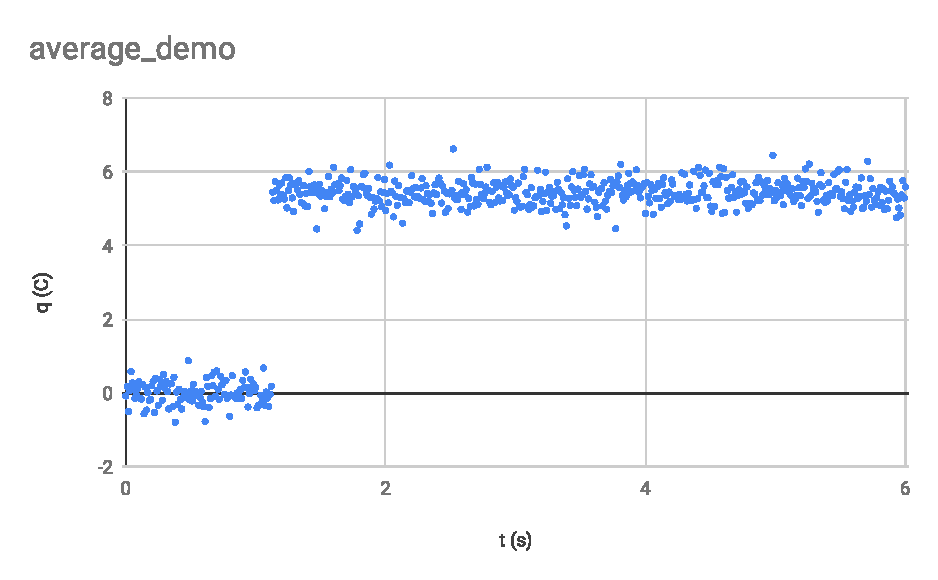
\includegraphics[scale=0.98]{image/00-review/average_demo.pdf}
    \caption{Part 1}
    \label{figure_00_average}
\end{figure}
\vspace{\stretch{1}}
%
\begin{figure}[ht]
    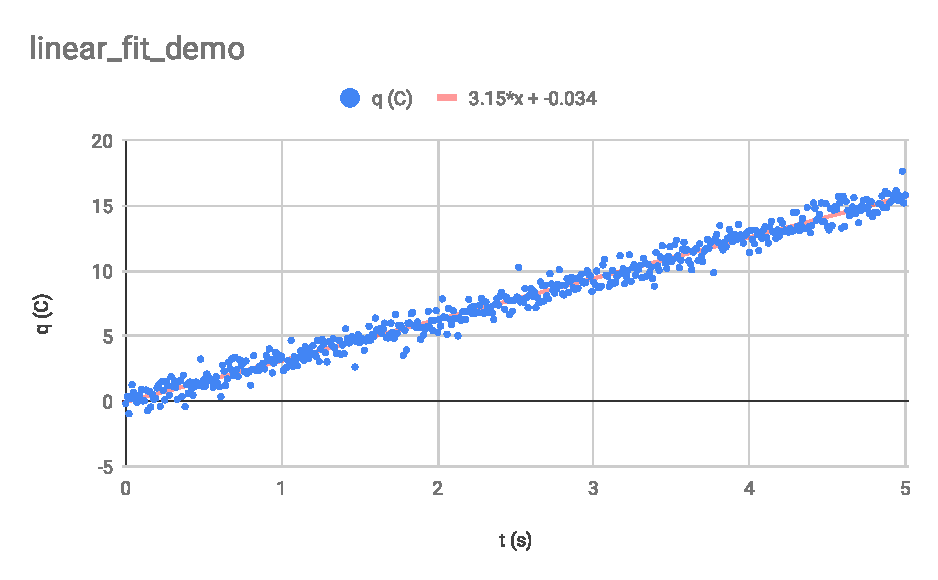
\includegraphics[scale=0.98]{image/00-review/linear_fit_demo.pdf}
    \caption{Part 2}
    \label{figure_00_linear}
\end{figure}
%
\begin{figure}[ht]
    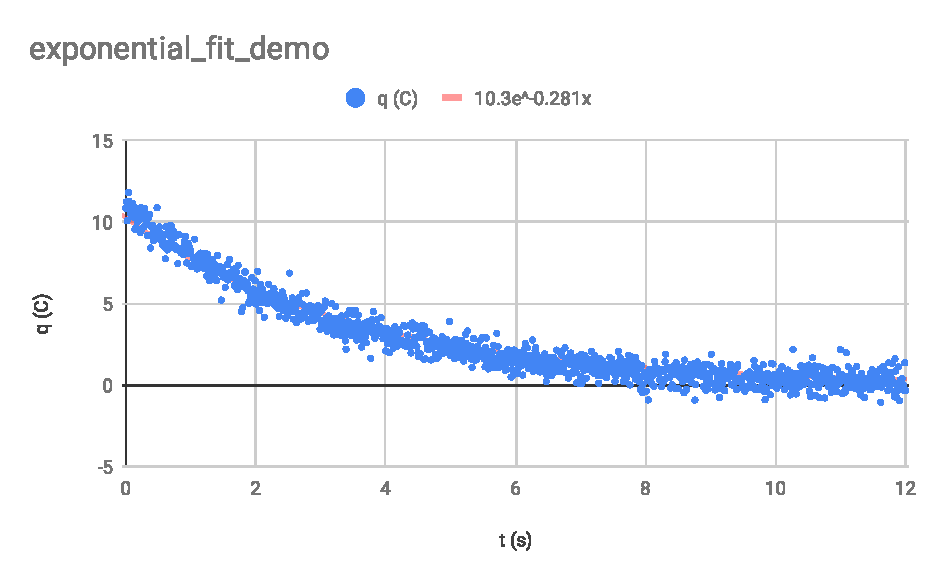
\includegraphics[scale=0.98]{image/00-review/exponential_fit_demo.pdf}
    \caption{Part 3}
    \label{figure_00_exponential}
\end{figure}
%